\documentclass[xcolor=dvipsnames]{beamer}
\usepackage{tikz,subcaption,amsmath,physics}
\usepackage{tikz-feynman}
\usetikzlibrary{shadings}
\setbeamercovered{highly dynamic}
% \tikzfeynmanset{compat=1.1.0}
\usetikzlibrary{shapes,arrows,decorations.pathmorphing,arrows.meta}
\usepackage{booktabs}
\usetheme{Madrid}
\useoutertheme[subsection=true,footline=authorinstitutetitle]{miniframes} % Alternatively: miniframes, infolines, split
\useinnertheme{circles}

% \definecolor{PrimeCol}{RGB}{21,96,100} % UBC Blue (primary)
% \definecolor{SecCol}{RGB}{0,196,154} % UBC Grey (secondary)
% \definecolor{AlertCol}{RGB}{244,96,54}
% \definecolor{PrimeCol}{RGB}{26,50,96}
\definecolor{PrimeCol}{RGB}{11, 79, 108}
% \definecolor{SecCol}{RGB}{69,203,232}
\definecolor{SecCol}{RGB}{31, 122, 140}

\definecolor{ThirCol}{RGB}{192,199,119}
\definecolor{AlertCol}{RGB}{241,127,41}





\setbeamerfont{author}{size=\Large}
\setbeamerfont{institute}{size=\normalsize\itshape}
\setbeamerfont{title}{size=\fontsize{30}{36}\bfseries}
\setbeamerfont{subtitle}{size=\Large\normalfont\slshape}



\setbeamercolor{palette primary}{bg=ThirCol,fg=white}
\setbeamercolor{palette secondary}{bg=SecCol,fg=white}
\setbeamercolor{palette tertiary}{bg=PrimeCol,fg=white}
\setbeamercolor{palette quaternary}{bg=black,fg=white}

\setbeamercolor{block title}{bg=PrimeCol,fg=white}
\setbeamercolor{block body}{bg=SecCol!10,fg=black}

\setbeamercolor{structure}{fg=PrimeCol} % itemize, enumerate, etc
\setbeamercolor{section in toc}{fg=PrimeCol} % TOC sections
\setbeamercolor{alerted text}{fg=AlertCol}
% Override palette coloring with secondary
\setbeamercolor{subsection in head/foot}{bg=SecCol,fg=white}
\setbeamercolor{frametitle}{fg=PrimeCol,bg=white}


\setbeamertemplate{title page}{%
\begin{tikzpicture}[remember picture,overlay,>=stealth',photon/.style={decorate,decoration={snake,post length=1mm}}]
\fill[PrimeCol]
  ([yshift=15pt]current page.west) rectangle (current page.south east);
\node[anchor=east] 
  at ([yshift=-30pt]current page.north east) (author)
  {\Huge\usebeamerfont{author}\color{PrimeCol} Gonçalo Garcês S.R. Baptista};
\node[anchor=north east] at ([yshift=-35pt]current page.north east)
{\footnotesize\color{PrimeCol} Bsc. in Physics Engineering};
\node[anchor=north east] at ([yshift=-50pt,xshift=.2cm]current page.north east){\footnotesize\color{PrimeCol}
\begin{tabular}{ r r}
 President:& Prof. André Wemans\\ 
 Rapporteur:& Prof. Jorge Sampaio\\  
 Advisor:& Prof. Mauro Guerra\\
 Co-Advisor:& Prof. Jorge Machado\\
\end{tabular}
};


\node[anchor=north east] 
  at ([yshift=-100pt]current page.north east) (institute)
  {\Large\usebeamerfont{institute} \color{PrimeCol} NOVA School of Science and Technology};
\node at ([yshift=-90pt,xshift=40pt]current page.north west) {\includegraphics[width=3cm]{NovaLogo.png}};

\node at ([yshift=-30pt,xshift=30pt]current page.north west) {\includegraphics[width=3.5cm]{logo_libphys.png}};




\node[anchor=east]
  at ([yshift=-10pt,xshift=-20pt]current page.east) (title)
  {\parbox[t]{.9\paperwidth}{\Large\color{white}X-ray Resonant Raman Scattering}};
\node[anchor=east]
  at ([yshift=-60pt,xshift=-20pt]current page.east) (subtitle)
  {\parbox[t]{.9\paperwidth}{\large\color{white} Spectra simulation from first principles\\for Copper below the ionization threshold\\ using high-performance computing}};

  \node at (current page.south east) [circle, draw, white, minimum size=10cm,dashed] {};
  
  \node at ([xshift=-3.54553390593cm,yshift=3.54553390593cm]current page.south east) [circle, draw,fill, white, minimum size=.5cm,opacity=.5] {};
  
  \node at (current page.south east) [circle, draw, white, minimum size=7.5cm,dashed]{} ;
  
  \node at ([xshift=-1.58481848cm,yshift=3.39865420cm]current page.south east) [circle, draw,fill, white, minimum size=.5cm,opacity=.5] {};
  
  \node at ([xshift=-0.3268340cm,yshift=3.735730cm]current page.south east) [circle, draw,fill, white, minimum size=.5cm,opacity=.5] {};
  
  \node at ([yshift=0.3268340cm,xshift=-3.735730cm]current page.south east) [circle, draw,fill, white, minimum size=.5cm,opacity=.5] {};
  
  \node at ([yshift=2.65165042945cm,xshift=-2.65165042945cm]current page.south east) [circle, draw,fill, white, minimum size=.5cm,opacity=.5] {};
  
  \node at ([yshift=1.58481848cm,xshift=-3.39865420cm]current page.south east) [circle, draw,fill, white, minimum size=.5cm,opacity=.5] {};
  
  \node at (current page.south east) [circle, draw, white, minimum size=5cm,dashed]{} ;
  
  \node at ([xshift=-2.5cm]current page.south east) [circle, draw,fill, white, minimum size=.5cm,opacity=.5] {};
  
  \node at ([yshift=2.5cm]current page.south east) [circle, draw,fill, white, minimum size=.5cm,opacity=.5] {};
  
  \node at ([xshift=-1.76777cm,yshift=1.76777cm]current page.south east) [circle, draw,fill, white, minimum size=.5cm,opacity=.5] {};
  
  \node at (current page.south east) [circle, draw, white, minimum size=2.5cm,dashed]{} ;
  
  \node at ([xshift=-0.8838835cm,yshift=0.8838835cm]current page.south east) [circle, draw,fill, white, minimum size=.5cm,opacity=.5] {};

  \draw[->,photon,white,opacity=.5] (current page.south east) -- node[below left] {} ([xshift=-5cm,yshift=5cm]current page.south east);

    \begin{feynman}
      % Specify your vertices using coordinates
      \vertex (a) at ([yshift=.3cm,xshift=3cm]current page.south west);
      \vertex [left =.375cm of a] (a1);
      \vertex [above =.75cm of a1] (a11);
      \vertex [left = .75cm of a1] (a2);
      \vertex [left = .75cm of a2] (a3);
      \vertex [right =.75cm of a] (b);
      \vertex [above =.75cm of b] (c);
      \vertex [above = .75cm of c] (d);
      \vertex [right = .75cm of b] (e);
      \vertex [right = .375cm of e] (f);
      \vertex [above = .75cm of f] (f1);
      \vertex [right = .75cm of f1] (f2);
      \vertex [right = .375cm of f2] (f3);
      \vertex [below = .75cm of f3] (f4);
      \vertex [right = .75cm of f4] (f5);
      % \vertex [right = .375cm of a] (point1);
      % \vertex [above = .375cm of point1] (point2);
      
      % Draw the Feynman diagram edges
      \diagram* {
        (a) -- [white,opacity=.5,half right,photon] (a2),
        (a2) -- [white,opacity=.5] (a3),
        (a) -- [white,opacity=.5] (b),
        (a) -- [white, opacity=.5] (a2),
        (b) -- [photon,white,opacity=.5] (c),
        (c) -- [fermion, half left,white,opacity=.5,looseness=1.8] (d),
        (d) -- [fermion, half left ,white,opacity=.5,looseness=1.8] (c),
        (b) -- [white, opacity=.5] (e),
        (e) -- [white, opacity=.5] (f),
        (e) -- [white, opacity=.5,quarter left,photon] (f1),
        (f1) -- [white, opacity=.5,half left,fermion,] (f2),
        (f2) -- [white, opacity=.5,half left,fermion] (f1),
        (f2) -- [white, opacity=.5,quarter left,photon] (f4),
        (f)  -- [white, opacity=.5] (f5),
      };
    \end{feynman};
  
\end{tikzpicture}
% \begin{tikzpicture}
%     \begin{feynman}
%     \vertex (i1) at (current page.south) ;
%     \vertex (f1) at (current page.south) ;
%     \diagram* {
%       i1[particle=$\ell$] --[fermion] f1 [particle=$i$]};
%   \end{feynman}
% \end{tikzpicture}
}



\author{Gonçalo Baptista}
\institute{NOVA School of Science and Technology}
\title{X-ray Resonant Raman Scattering}
\subtitle{Linguistics as a Window for Understanding the Brain}



%%%%%%%%%%%%%%
\setbeamertemplate{bibliography item}{\insertbiblabel} %% Remove book symbol from references and add number
\usepackage[style=ieee,backend=bibtex,citetracker=true]{biblatex}
\addbibresource{bibliography.bib}










\newcommand<>{\uncovergraphics}[2][{}]{
    % Taken from: <https://tex.stackexchange.com/a/354033/95423>
    \begin{tikzpicture}
    \node[anchor=south west,inner sep=0] (B) at (4,0)
        {\includegraphics[#1]{#2}};
    \alt#3{}{%
        \fill [draw=none, fill=white, fill opacity=0.9] (B.north west) -- (B.north east) -- (B.south east) -- (B.south west) -- (B.north west) -- cycle;
    }
    \end{tikzpicture}
}



% \title[Title Without Rambling]{My Rambling Presentation Title}
% \date{\today}
% \author[G.B.]
% {Gonçalo Garcês Sobreira Rodrigues Baptista}
% \institute[NOVA-SST]{RamblingAcademic.com\\Nuts and Bolts of Research. Plus Some Rambling.}
\AtBeginSection[]
{
 \begin{frame}<beamer>
 \frametitle{Overview}
    \begin{columns}[T]
        \begin{column}{.45\textwidth}
            \tableofcontents[currentsection,sections=1-2]
        \end{column}
        \begin{column}{.45\textwidth}
            \tableofcontents[currentsection,sections=3-]
        \end{column}
    \end{columns}
 \end{frame}
}

\makeatletter
\let\beamer@writeslidentry@miniframeson=\beamer@writeslidentry%
\def\beamer@writeslidentry@miniframesoff{%
  \expandafter\beamer@ifempty\expandafter{\beamer@framestartpage}{}% does not happen normally
  {%else
    % removed \addtocontents commands
    \clearpage\beamer@notesactions%
  }
}
\newcommand*{\miniframeson}{\let\beamer@writeslidentry=\beamer@writeslidentry@miniframeson}
\newcommand*{\miniframesoff}{\let\beamer@writeslidentry=\beamer@writeslidentry@miniframesoff}
\makeatother

\begin{document}
	
	\begin{frame}[plain]
		\titlepage
	\end{frame}
	

	
	\section{Theoretical Introduction}
    \subsection{Characteristic x-rays}
    \begin{frame}{X-ray applications}
        \begin{figure}[h!]
            \centering\hfill
            \begin{subfigure}{0.3\textwidth}
            \uncovergraphics<1->[width=\linewidth]
            {medical_xray.jpg}
            \uncover<1->{\caption{Imaging purposes}}
            \end{subfigure}
            \begin{subfigure}{0.33\textwidth}
            \uncovergraphics<2->[width=\linewidth]{500uL.pdf}
            \uncover<2->{\caption{Sample quantification}}
            \end{subfigure}\hfill
            \begin{subfigure}{0.33\textwidth}
            \uncovergraphics<3->[width=\linewidth]
            {KAlpha.pdf}
            \only<1-3>{\uncover<3->{\caption{Fundamental parameters}}}
            \only<4>{\caption{\alert{Fundamental parameters}}}
            \end{subfigure}\hfill
            \caption{Application examples of x-ray radiation}
        \end{figure}
    \end{frame}

\begin{frame}{Vacancy generation and relaxation processes}
\begin{columns}[T,onlytextwidth]
    \column{0.5\textwidth}
    \begin{center}\vspace{-1cm}
    \begin{tikzpicture}[>=stealth',photon/.style={decorate,decoration={snake,post length=1mm}}]
        \draw (0,0) -- (0,1);
        \draw (0,1.2) -- (0,5);
        \draw[-Stealth] (0,5.2) -- (0,6);
        \shade[bottom color=black, top color= white] (0.2,5.3) rectangle (4.2,6);
        
        \draw (-0.1,4.9) -- (0.1,5.1);
        \draw (-0.1,5.1) -- (0.1,5.3);
        \draw (-0.1,0.9) -- (0.1,1.1);
        \draw (-0.1,1.1) -- (0.1,1.3);
        \node[anchor=east,align=center] at (-0.1,0.5) {Inner\\shell};
        \node[anchor=east,align=center] at (-0.1,2.7) {Outer\\shells};
        \node[anchor=east] at (0,6) {$E$};
        
        \draw (0.2,0.5) -- (4.2,0.5);
        \draw (-0.1,0.5) -- (0.1,0.5);
        \draw (.2,2)   --  (4.2,2);
        \draw (.2,2.7)   --  (4.2,2.7);
        \draw(.2,4)  -- (4.2,4);

        
        \draw[fill=SecCol](0.2+4/3,0.5)circle (.2cm);
        \only<1,2,6->{\draw[fill=SecCol](0.2+8/3,0.5)circle (.2cm)};
        \draw[fill=SecCol](0.2+4/3,2)circle (.2cm);
        \only<1-5>{\draw[fill=SecCol](0.2+8/3,2)circle (.2cm)};
        \draw[fill=SecCol](0.2+4/3,2.7)circle (.2cm);
        \draw[fill=SecCol](0.2+8/3,2.7)circle (.2cm);
        \only<-6>{\draw[fill=SecCol](0.2+4/3,4)circle (.2cm)};
        \draw[fill=SecCol](0.2+8/3,4)circle (.2cm);

        \only<3,4,5>{\draw[fill=SecCol,opacity=.3,dashed](0.2+8/3,0.5)circle (.2cm)};
        \only<6->{\draw[fill=SecCol,opacity=.3,dashed](0.2+8/3,2)circle (.2cm)};
        \only<3,7>{\draw[fill=SecCol](0.2+6/3,6)circle (.2cm)};
        \only<7>{\draw[fill=SecCol,dashed,opacity=.3](0.2+4/3,4)circle (.2cm)};

        \only<7>{\draw[-Stealth] (.2+4/3,4.2) .. controls (2.2,5) .. (2.2,5.8)};
        \only<3>{\draw[-Stealth] (.2+8/3,.7) .. controls (.2+2,1.7) .. (2.2,5.8)};
        \only<2>{\draw[photon,-Stealth] (4.5,1.5)--(3.,1)};
        \only<6>{\draw[photon,-Stealth](.2+8/3,1.25)-- (4,2.5)};
        \only<6->{\draw[-Stealth](.2+8/3,1.8)--(.2+8/3,.7)};
        
    \end{tikzpicture}
    \end{center}
    \column{0.5\textwidth}
    \begin{itemize}
        \uncover<1>{\item Bound state system}
        \uncover<2>{\item Energy transfer}
        \uncover<3>{\item Ionization}
        \uncover<4>{\item Vacancy generated}
        \uncover<5->{\item Atomic Relaxation\begin{itemize}
            \uncover<6>{\item Radiative relaxation (x-ray emission)}
            \uncover<7>{\item Auger electron emission}
        \end{itemize}}
    \end{itemize}
\end{columns}
\end{frame}

\begin{frame}{Alternative processes}
\begin{block}{Shake processes}
   Post-ionization, the different number of particles in the system leads to a change in the Hamiltonian. This leads to the lack of orthogonality between non-equivalent states and free-wave wavefunctions in the initial and final configurations.
       % \begin{equation}
       %     \hfill\uncover<2->{\braket{1\text{s}_\text{i}}{2\text{s}_\text{f}}\neq 0}\qquad \uncover<3->{ \braket{1\text{s}_\text{i}}{e^{-}_\text{free}}\neq 0}
       % \end{equation}
      \begin{equation*}
           \hfill\braket{1\text{s}_\text{i}}{2\text{s}_\text{f}}\neq 0  \qquad\braket{1\text{s}_\text{i}}{e^{-}_\text{free}}\neq 0
       \end{equation*}
\end{block}




\begin{columns}[T,onlytextwidth]
    \column{0.45\textwidth}
    \uncover<2>{\begin{block}{Shake-up}
        Excitation of extra electron(s).
    \end{block}}
    \column{0.45\textwidth}
    \uncover<3>{\begin{block}{Shake-off}
        Ionization of extra electron(s).
    \end{block}}
\end{columns}

\begin{tikzpicture}[overlay,remember picture]
\only<2>{\draw[line width=.5mm,color= PrimeCol] ([xshift=-3cm,yshift=-1.2cm]current page.center) -- ([xshift=-5cm,yshift=-1.2cm]current page.center)};
\only<2>{\draw[line width=.5mm,color= PrimeCol,-Stealth] ([xshift=-5cm,yshift=-1.2cm]current page.center) -- ([xshift=-5cm,yshift=-2cm]current page.center)};

\only<3>{\draw[line width=.5mm,color= PrimeCol] ([xshift=3cm,yshift=-1.2cm]current page.center) -- ([xshift=5cm,yshift=-1.2cm]current page.center);
\draw[line width=.5mm,color= PrimeCol,-Stealth] ([xshift=5cm,yshift=-1.2cm]current page.center) -- ([xshift=5cm,yshift=-2cm]current page.center);}


\end{tikzpicture}
\end{frame}

\begin{frame}[c]{Alternative processes}
\begin{columns}[T,onlytextwidth]
\column{0.45\textwidth}

    \begin{block}{Shake Processes}
    The probability of these processes occurring is extremely dependent on the incident energy.

    Since for this thesis, the energy ranges studied were below the ionization threshold, no shake processes were accounted for.
\end{block}
\column{0.45\textwidth}
\vspace{-1.2cm}
\begin{figure}
    \centering
    \includegraphics[width=.9\linewidth]{thomas_model.png}
    \caption{Thomas model for shake probability.~\cite{PhysRevLett.52.417}}
    
\end{figure}
    
\end{columns}
\end{frame}


\begin{frame}{Other processes}
    \begin{columns}[T,onlytextwidth]
    \column{0.45\textwidth}
    \begin{block}{Photoexcitation}
        The most relevant process, for the scope of this work, is that of resonant photoexcitation.
        In it, instead of a vacancy generated due to sending one electron to the continuum, it has, in turn, remained bound but in a higher energy level.
    \end{block}
    \column{0.45\textwidth}
        \begin{center}\vspace{-1cm}
    \begin{tikzpicture}[>=stealth',photon/.style={decorate,decoration={snake,post length=1mm}}]
        \draw (0,0) -- (0,1);
        \draw (0,1.2) -- (0,5);
        \draw[-Stealth] (0,5.2) -- (0,6);
        \shade[bottom color=black, top color= white] (0.2,5.3) rectangle (4.2,6);
        
        \draw (-0.1,4.9) -- (0.1,5.1);
        \draw (-0.1,5.1) -- (0.1,5.3);
        \draw (-0.1,0.9) -- (0.1,1.1);
        \draw (-0.1,1.1) -- (0.1,1.3);
        \node[anchor=east,align=center] at (-0.1,0.5) {Inner\\shell};
        \node[anchor=east,align=center] at (-0.1,2.7) {Outer\\shells};
        \node[anchor=east] at (0,6) {$E$};
        
        \draw (0.2,0.5) -- (4.2,0.5);
        \draw (-0.1,0.5) -- (0.1,0.5);
        \draw (.2,2)   --  (4.2,2);
        \draw (.2,2.7)   --  (4.2,2.7);
        \draw(.2,4)  -- (4.2,4);

        
        \draw[fill=SecCol](0.2+4/3,0.5)circle (.2cm);
        \only<1,2>{\draw[fill=SecCol](0.2+8/3,0.5)circle (.2cm)};
        \draw[fill=SecCol](0.2+4/3,2)circle (.2cm);
        \only<1->{\draw[fill=SecCol](0.2+8/3,2)circle (.2cm)};
        \draw[fill=SecCol](0.2+4/3,2.7)circle (.2cm);
        \draw[fill=SecCol](0.2+8/3,2.7)circle (.2cm);

        \draw[fill=SecCol](0.2+8/3,4)circle (.2cm);

        \only<3>{\draw[fill=SecCol,opacity=.3,dashed](0.2+8/3,0.5)circle (.2cm)};




        \only<3>{\draw[fill=SecCol](0.2+4/3,4)circle (.2cm)};
        \only<3>{\draw[-Stealth] (.2+8/3,.7) .. controls (.2+2,1.7)  .. (.2+4/3,3.8)};
        \only<2>{\draw[photon,-Stealth] (4.5,1.5)--(3.,1)};
        
    \end{tikzpicture}
    \end{center}
    \end{columns}
\end{frame}
    
    \subsection{The Hamiltonian}

    \begin{frame}[c]{Schrödinger's Hamiltonian}

    In its most basic form, for a "classical" atom (nucleus + electrons), and when relativistic effects are not taken into account, the considered Hamiltonian follows the one use in Schrödinger's equation:

    \begin{equation*}
        \hat{H}=\displaystyle \sum_i^N\only<1,3->{\frac{1}{2}\laplacian_i}\only<2>{{\color{AlertCol}\frac{1}{2}\laplacian_i}} \only<1-2,4->{- \frac{Z}{r_i}} \only<3>{{\color{AlertCol}- \frac{Z}{r_i}}} + \sum_{j>i}\only<1-3>{ \frac{1}{r_{ij}}}\only<4>{{\color{AlertCol}+ \frac{1}{r_{ij}}}}
    \end{equation*}
    
    \uncover<2->{It incorporates:
    \begin{itemize}
        \only<1,3->{\item The kinetic energy of the electron.}
        \only<2>{\item {\color{AlertCol}The kinetic energy of the electron.}}
        
        \only<1,2,4>{\item The potential energy of the electron-nucleus attraction.}
        \only<3>{{\color{AlertCol}\item The potential energy of the electron-nucleus attraction.}}
        
        \only<1-3>{\item  The potential energy of the electron-electron repulsion.}
        \only<4>{{\color{AlertCol}\item  The potential energy of the electron-electron repulsion.}}
        
    \end{itemize}}
    \end{frame}

    \begin{frame}[c]{Solving the non-relativistic many-body problem}
        \begin{columns}[T,onlytextwidth]
        \column{0.45\textwidth}
        \only<1-7>{\begin{block}{}
            Due to the complexity introduced by the many bodies in the system, and their interactions, a numerical method needs to be employed as to obtain eigenfunctions for this Hamiltonian.
        \end{block}}
        
        \only<8>{
        \begin{block}{}
            Each of the electrons' wavefunctions, $u$, are composed as a product of a spatial part, $\psi$, and one related to the electron's spin $\chi$.
            \begin{equation*}
                u=\psi \chi
            \end{equation*}
            The system's wavefunction should then be written as a Slater determinant as to account for anti-symetry and the fermionic nature of the electrons.
        \end{block}}
        \only<9>{
        \begin{block}{}
            Through a {\color{AlertCol}self-consistent} field approach, the method solves, for each cycle, a set of integro-differential equations as a way to compute new wavefunctions and the new energy for the system.
        \end{block}
        }
        \only<10>{
        \begin{block}{}
            This process is then repeated up until the energy difference in-between two steps is under a pre-defined benchamark value, as to assure the computation has converged.
        \end{block}
        }

        \column{0.5\textwidth}
        \only<10>{
            METER DIAGRAMA DE BLOCOS
        }
        
        \only<1-7>{
        \begin{center}\vspace{-1cm}
        \begin{tikzpicture}[>=stealth',photon/.style={decorate,decoration={snake,post length=1mm}}]


        \only<3-7>{\draw[photon,->]  (0,0) -- (0,1.2);}
        \only<5-7>{\draw[photon,->]  (0,0) -- (0.707106781*2,0.707106781*2);}
        \only<7>{\draw[photon,->]  (-0.707106781*3,0.707106781*3) -- (0.707106781*2,0.707106781*2);}
        \only<7>{\draw[photon,->]  (-0.707106781*3,0.707106781*3) -- (0,1);}
        \only<5-7>{\draw[photon,->]  (0.707106781*2,0.707106781*2) -- (0,1);}
        \only<7>{\draw[photon,->]  (0,0) -- (-0.707106781*3,0.707106781*3);}

        
        \draw[color=PrimeCol] (0,0) circle (1cm);
        
        \draw[fill=AlertCol,dashed] (0,0) circle (.3cm);
        \uncover<2->{\draw[fill=SecCol]  (0,1) circle (.2cm);}
        \draw[color=PrimeCol] (0,0) circle (2cm);
        \uncover<4->{\draw[fill=SecCol]  (0.707106781*2,0.707106781*2) circle (.2cm);}
        \draw[color=PrimeCol] (0,0) circle (3cm);
        \uncover<6->{\draw[fill=SecCol]  (-0.707106781*3,0.707106781*3) circle (.2cm);}


        \end{tikzpicture}

        \end{center}}
        \only<9>{
        \begin{center}
        \vspace{-1cm}
        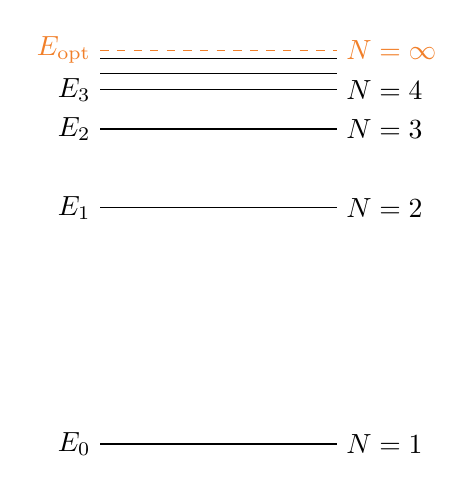
\begin{tikzpicture}
            \node[anchor=east] at (0,0) {$E_0$};
            \node[anchor=east] at (0,3) {$E_1$};
            \node[anchor=east] at (0,4) {$E_2$};
            \node[anchor=east] at (0,4.5) {$E_3$};
            \node[anchor=east,color=AlertCol] at (0,5) {$E_\text{opt}$};

            \node[anchor=west] at (3,0) {$N=1$};
            \node[anchor=west] at (3,3) {$N=2$};
            \node[anchor=west] at (3,4) {$N=3$};
            \node[anchor=west] at (3,4.5) {$N=4$};
            \node[anchor=west,color=AlertCol] at (3,5) {$N=\infty$};
            
            \draw (0,0) -- (3,0);
            \draw (0,3) -- (3,3);
            \draw (0,4) -- (3,4);
            \draw (0,4.5) -- (3,4.5);
            \draw (0,4.7) -- (3,4.7);
            \draw (0,4.9) -- (3,4.9);
            \draw[dashed,color=AlertCol] (0,5) -- (3,5);
        \end{tikzpicture}
            
        \end{center}
        }       

        \only<8>{
        \vspace{1cm}
        \begin{equation*}
            \frac{1}{\sqrt{N!}}\mqty|u_1\qty(x_1)&u_2\qty(x_1)&\hdots&u_N\qty(x_1)\\
                                    u_1\qty(x_2)&u_2\qty(x_2)&\hdots&u_N\qty(x_2)\\
                                    \vdots  &   \vdots  &   \ddots  &   \vdots\\
                                    u_1\qty(x_N)&u_2\qty(x_N)&\hdots&u_N\qty(x_N)|
        \end{equation*}
        }
        \end{columns}
    \end{frame}

    \begin{frame}{Limitations of the non-relativistic approach}

    \begin{columns}[T,onlytextwidth]
    \column{0.45\textwidth}
    While Schrodinguer's equation may be quite accurate for low energy systems (e.g. Hydrogen), where the speed of the surrounding electrons is not comparable to that of light, such is not the case for more complex and heavier systems.
    
    \column{0.45\textwidth}
    \begin{block}{Speed of 1s electrons in ground state configurations (\% of $c$)}
        \begin{tabular}{lr}
            Hydrogen:&$0.516\%$\\
            \alert{Copper:}&{\color{AlertCol}$14.883\%$}
        \end{tabular}
    \end{block}





    \end{columns}
    \end{frame}


    
    \subsection{State-of-the-art}
    \section{Atomic structure calculations}
    \subsection{The system at study}
    \subsection{Level calculations}
    \subsection{Transition computations}
    \subsection{Fundamental atomic parameters}
    \section{Spectra simulation}
    \subsection{Line shape}
    \subsection{Photoexcitation}
    \subsection{Photoionization}
    \subsection{The synthetic spectrum}
    \section{Spectral Analysis}
    \subsection{The theoretical results}
    \subsection{Comparison with experimental data}
    \section{A new parallelization code}
    \subsection{The MPI approach}
    \subsection{Speedup comparison}
    \miniframesoff
    \appendix
    \section*{+}
 \begin{frame}{Conclusion}
     
 \end{frame}

 \begin{frame}[plain]{}
 \begin{center}
     \Huge Thank you\\
     for your attention!
 \end{center}

 
      \begin{tikzpicture}[remember picture,overlay]
      
         \begin{feynman}
             \vertex (a0) at ([yshift=1.5cm,xshift=-3cm]current page.south);
             \vertex[right=1cm of a0] (a1);
             \vertex[right=1cm of a1] (a2);
             \vertex[above=1.5cm of a2] (a3);
             \vertex[right=2cm of a3] (a4);
             \vertex[right=3cm of a2] (a5);
             \vertex[right=1cm of a5] (a6);
             \vertex[above=.5cm of a3] (v1);
             \vertex[right=.15cm of v1] (v2);
             \vertex[left=.15cm of a4] (v3);
             \vertex[below=.5cm of v3] (v4);
             \vertex[below=.16667cm of v2] (b1);
             \vertex[right=.28cm of b1] (b2);
             \vertex[right=.28cm of b2] (b3);
             \vertex[below=.16667cm of b3] (b4);
             \vertex[above=.16667cm of v4] (c1);
             \vertex[left=.28cm of c1] (c2);
             \vertex[above=.16667cm of c2] (c3);
             \vertex[left=.28cm of c3] (c4);
             \vertex[left=.1cm of v2] (m1);
             \vertex[below=.2cm of m1] (m2);
             \vertex[left=.23cm of v4](m3);
             \vertex[below=.2cm of m3](m4);
             \diagram*{
             % (a0) -- (a2),
             (a1) --[photon,quarter left](a3),
             (a3) --[half left](a4),
             (a3) --[half right](a4),
             (a0) --[fermion] (a6),
             (a4) --[photon,quarter left](a5),
             % (a5) -- (a6),
             (v2) --[photon] (b2),
             (c4) --[photon] (b4),
             (v4) --[photon] (c2),
             % (b3) -- (b4)
             (b2) -- [half left] (b4);
             (b2) -- [half right] (b4);
             (c2) -- [half left] (c4);
             (c2) -- [half right] (c4);
             (m4) --[photon,quarter left] (m2);
             };
             
         \end{feynman}
     \end{tikzpicture}
     
 \end{frame}


\end{document}